


\subsection*{Exercice 1 : Mise hors gel des canalisations d'eau (temps : 45 min – difficulté : $\star\star $)}

La température dans le sol terrestre étant initialement constante, égale à 5\textdegree C , on cherche à déterminer
à quelle profondeur minimale il est nécessaire d’enterrer une canalisation d’eau pour qu’une brusque
chute de la température de sa surface à -15\textdegree C n’entraine pas le gel de cette canalisation après 10 jours.



%\begin{minipage}[c]{.6\linewidth}
Les hypothèses sont les suivantes :
\begin{itemize}
\item la température en un point quelconque du sol et de sa surface à tout instant $t < 0$ est constante et égale à $T_0=278\;K$ ( $\theta_0=5^oC$ ) ;
\item la température à la surface du sol, confondue avec le plan d’équation $z = 0$, passe brutalement à l’instant $t = 0$ , de $T_0 = 278\;K$ à $T_1 =  258\; K$ ($\theta_1 = -15^o C$) et se maintient à cette valeur pendant
$t_f= $10 jours.
\end{itemize}
\begin{center}
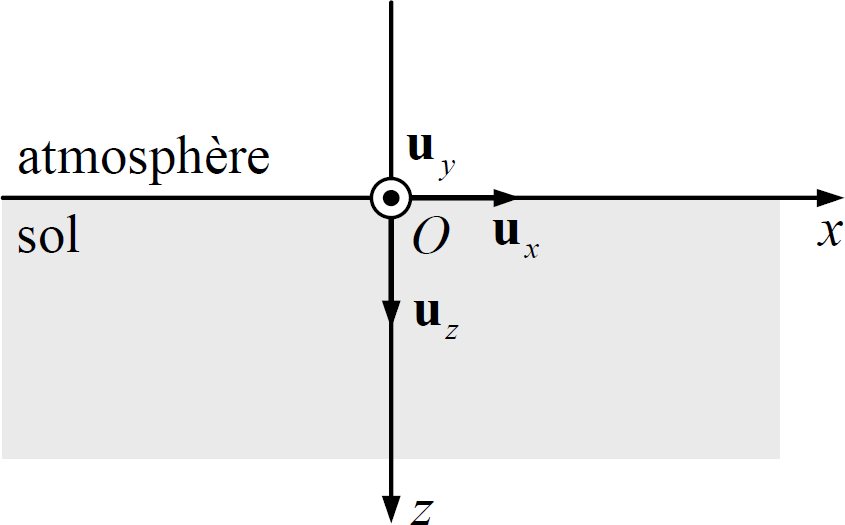
\includegraphics[width=.95\linewidth]{images/canalisation}
\end{center}
On peut montrer que la température $T(z, t)$ à la profondeur $z$ et à l’instant $t$ est donnée par la relation suivante :

$$
T(z,t)=T_1 + (T_0-T_1) \text{erf}\left( \dfrac{z}{2\sqrt{Dt}} \right)
$$
où $\text{erf}(x)$ désigne la fonction définie par :
$$
\text{erf}(x) = \dfrac{2}{\sqrt{\pi}}\int^x_0 e^{-u^2} \mathrm{d}u
$$

Données numériques : $D=2,8\cdot 10^{-7} \; m^2\cdot s^{-1}$ (diffusivité thermique du sol terrestre).

\setcounter{subparagraph}{0}

\subparagraph{}
\textit{Écrire une fonction python, appelée \texttt{integrale}, permettant de réaliser d'intégrer une fonction sur un intervalle, en utilisant la méthode du point milieu.}

\subparagraph{}
\textit{Écrire une fonction Python, appelée \texttt{erf}, prenant en paramètre un nombre réel positif ou nul $x$ et retournant la valeur de \texttt{erf(x)}.}

\subparagraph{}
\textit{Écrire une fonction Python, appelée \texttt{Temperature}, prenant en paramètre la profondeur $z$ (exprimée en $m$) et le temps $t$ (exprimé en $s$) et retournant la valeur de la température $T(z, t)$.}

\subparagraph{}
\textit{Écrire un programme Python permettant de créer une liste, nommée \texttt{ListeErreur}, contenant les valeurs de la fonction \texttt{erf(x)} pour $x$ variant par pas de 0,05 dans l’intervalle $[0 ; 2]$.}

\subparagraph{}
\textit{En déduire, à 1 cm près, à quelle profondeur minimale $z_{min}$ il est nécessaire d'enterrer une canalisation d'eau pour qu'une brusque chute de la température de la surface du sol de 5\textdegree C à -15 \textdegree C n'entraine pas le gel de cette canalisation au bout de 10 jours.}
